% Define document class. Important.
\documentclass[a4paper,twoside,openany]{report}

% Margener
%\setlength{\evensidemargin}{1cm}
%\setlength{\oddsidemargin}{1cm}

% Set up encoding. Latin1 since UTF-8 is fuckably difficult to work with.
% \usepackage[latin1]{inputenc}
\usepackage[latin1,utf8,ansinew]{inputenc}

% Variable, neat, references.
\usepackage{varioref}

% Load up bibliography.
\usepackage{natbib}
% Bibliography style.
\bibliographystyle{plain}

% Algorithm support.
\usepackage{algorithmic}
\usepackage{algorithm}
% Make algorithms appear as procedures instead.
\floatname{algorithm}{Procedure}
\renewcommand{\algorithmicrequire}{\textbf{Input:}}
\renewcommand{\algorithmicensure}{\textbf{Output:}}

% Image frames.
\setlength{\fboxsep}{0pt}
\setlength{\fboxrule}{0.5pt}

% Also, images.
\usepackage{graphicx}

% Todo notes here and there.
\usepackage[disable]{todonotes}

% Forbedrede floats.
\usepackage{float}

% Special symbols availability.
\usepackage{amssymb}

% CODE %
\usepackage{listings}
\usepackage{color}
\definecolor{gray}{rgb}{0.4,0.4,0.4}
\definecolor{darkblue}{rgb}{0.0,0.0,0.6}
\definecolor{cyan}{rgb}{0.0,0.6,0.6}
\lstset{
  basicstyle=\ttfamily,
  columns=fullflexible,
  showstringspaces=false,
  commentstyle=\color{gray}\upshape,
  basicstyle=\small,
  numberstyle=\footnotesize,
  numbers=left,
  captionpos=b,
  stepnumber=1,
  numbersep=10pt,
  tabsize=2,
  breaklines=true,
}
% Define markup of XML
\lstdefinelanguage{XML}
{
  morestring=[b]",
  morestring=[s]{>}{<},
  morecomment=[s]{<?}{?>},
  identifierstyle=\color{darkblue},
  keywordstyle=\color{cyan},
  morekeywords={id, target, type, category, value, point, correct, rows, width, time}% list your attributes here
}
% Define markup of C#
\lstdefinelanguage{CSharp}[Visual]{C++}
{
	identifierstyle=\color{darkblue},
	commentstyle=\color{green!70!black}\itshape ,
	stringstyle=\color{gray},
	sensitive=true,
	morestring=[b]",
	morestring=[b]',
	morecomment=[l]//,
	morecomment=[n]{/*}{*/}
}

% Neat-o referencer...o.
\usepackage{hyperref}
\usepackage{nameref}

% hack fra nettet.
% http://tex.stackexchange.com/questions/1230/reference-name-of-description-list-item-in-latex
\makeatletter
\let\orgdescriptionlabel\descriptionlabel
\renewcommand*{\descriptionlabel}[1]{%
  \let\orglabel\label
  \let\label\@gobble
  \phantomsection
  \edef\@currentlabel{#1}%
  %\edef\@currentlabelname{#1}%
%  \let\label\orglabel
  \orgdescriptionlabel{#1}%
}
\makeatother
% Rettehak. Meget lettere end \checkmark
\newcommand{\yes}{\checkmark}

% Let's put in a lot of niceness in the display, yeh?
\usepackage{fancyhdr} % Get some niceness into our headers.
\pagenumbering{arabic} % Ensure page numbering in our desired form.
\pagestyle{fancy}
% Page design from fancyhdr.
\fancyhead{}
\fancyfoot{}
\fancyhead[RO,LE]{\leftmark\\\rightmark}
\fancyfoot[C]{\thepage}
\setlength{\headheight}{23pt}
% Rewrite header and footer commands.
\renewcommand{\headrulewidth}{1.0pt}
\renewcommand{\footrulewidth}{1.0pt}

% Create a new command, HRule, to insert some nice horisontal rules on the title page.
\newcommand{\HRule}{\rule{\linewidth}{0.3mm}}

% New command for two figures, side by side.
\newcommand{\twofigs}[6]
{
	\begin{figure}[H]
		\begin{minipage}[b]{0.5\columnwidth}
		\centering\fbox{\includegraphics[width=0.8\columnwidth]{img/#1}}\caption{#2\label{#3}}
		\end{minipage}
		\hspace{0.5cm}
		\begin{minipage}[b]{0.5\columnwidth}
		\centering\fbox{\includegraphics[width=0.8\columnwidth]{img/#4}}\caption{#5\label{#6}}
		\end{minipage}	\end{figure}
}

% Sørg for at paragrafplads ikke spildes.
\raggedbottom

\begin{document}

\thispagestyle{empty}
\begin{center}
	%\includegraphics[width=15cm]{forside.png}\\~\\
	\hrulefill\newline
	\\
	\begin{LARGE}	
	\textbf{GIRAF Admin}
	\end{LARGE}
	\\
	\begin{large} 
	\textbf{An administrative addition to the GIRAF framework}
	\end{large}\\
	\hrulefill\newline
	%\hrule
	\\~\\
	Aalborg University, Second year in Engineering, Science and Medicine\\
	SW3, fall semester 2011	\\
	Project group SW305E11\\
\end{center}

\newpage
\thispagestyle{empty}
\mbox{}

%\newpage
%\thispagestyle{empty}
%\mbox{}

%\newpage
%\thispagestyle{empty}
%\mbox{}
%\fancyhead{}
%\fancyfoot{}
%\fancyhead[RO,LE]{\leftmark\\\rightmark}
%\fancyfoot[C]{\thepage}
%\setlength{\headheight}{23pt}

% Fjern headeren for indholdsfortegnelsen.
%\fancyhead{}
%\fancyfoot{}
%\fancyhead[RO,LE]{\leftmark}
%\fancyfoot[C]{\thepage}
%\setlength{\headheight}{23pt}% Indholdsfortegnelser etc.
% Dybde for visning af niveauer.
% Dybde af niveaut�lling generelt.
\setcounter{secnumdepth}{3}
\setcounter{tocdepth}{1}

\tableofcontents

% 1. Introduktion & analyse
\part{Analysis}

%kapitel introduction
\chapter{Introduction}

In our project we have had contact with Birken which is a kindergarten for special-needs children, which is located at Vodskov in Northern Denmark region.
Our contact from Birken, Kristine Niss-Henriksen has been included in this project because of her knowledge about children with autism and experience with today's technology.
With her help we were able to get a different view on things and new ideas for our program. We also got her to test our first functional prototype, which helped us form our final product.  

Some words are defined in the list below for the reader's convenience
\begin{itemize}
\item{Guardians = Parents}

\end{itemize}

\section{Autism}
Autism is defined as a developmental disorder, which effects the brain's ability to develop communication- and social skills. Autism often appears during the first three years of a child's life, and the disorder is often diagnosed during the following years.
The definition of autism is broad, which means that some autistic children have different symptoms than their peers, but to diagnose, the \textit{Autism Spectrum Disorder} which consists of three basic symptoms, is used. These three symptoms are listed below.
\begin{itemize}

  \item{Lack of communications skills.}
   \begin{itemize}
     \item{The child has slow or no development of language. The child may use gestures to communicate instead of words, it may have trouble with maintaining focus in a conversation or have trouble starting a conversation.}
   \end{itemize}
   
  \item{Lack of social skills.}
   \begin{itemize}
     \item{The child may have difficulty making friends. The child may be withdrawn or may not respond to eyecontact and smiles. The child may treat other children and/or adults as objects. The child may rather play alone than play with others.}
   \end{itemize}

  \item{Repetitive and/or compulsive behavior}
    \begin{itemize}
      \item{The child may have unusual distress if particular routines are changed or not being followed. The child may perform repeated body movements. \cite{autism}}
    \end{itemize}
  
\end{itemize}

The exact causes of autism are still unknown, but are supposedly a combination of different factors. Some possible causes, which have been suspected though not proven, are listed below:

\begin{itemize}
  
  \item{Diet}
  \item{Changes of the digestive tract}
  \item{Poison by mercury}
  \item{The body's lack of ability to utilize vitamins and minerals properly}
  \item{Sensitivity against vaccines\cite{autism}}
  
\end{itemize}

Even though the factors listed above are mostly physical, the autism disorder is supposedly linked to unusual biology and the chemistry of the brain.
It seems that genetics are an important factor. E.g. it is more likely for identical twins, than fraternal twins or siblings, to both be autistic\cite{autism}.
\section{Communication with an autistic child}
The parent and kindergarten teachers use Picture Exchange Communication System or \textit{PECS}, to communicate with an autistic child and this system has been successfully used for over 10 years in the USA. The communication tool consists of pictures or pictograms that represent something, the child is to do or wants to do. This can be a drawing of an apple, signaling the child which fruit to eat. 

This form of communication is used within kindergartens for children with special needs e.g. children with autism. Mostly these pictograms are printed from a computer program called Boardmaker, which has many different pictograms that can be edited to make it easier for the child to understand. This could be when the child needs to put on a blue t-shirt, then the adult gives the child a pictogram of a blue t-shirt and the child understands. It can be confusing for the child if the actual t-shirt is one color and the one on the pictogram is another.

The PECS can also be used as a schedule for the children. In the kindergarten \textit{Birken}, pictograms are used as a daily schedule, where Kindergarten teachers put the pictograms on the wall so one row represents the activities of the day. Then the kindergarten teacher teaches the child to take the pictogram of the finished activity and put it away in a box. Later the pictogram can be put on next day's schedule, without confusing the child about whether the activity is finished or not.
%Later in the child's development the pictogram would be put next to the schedule, but the child would still understand that this activity is finished.


%kapitel problem analyse
\chapter{Problem analysis}

In this chapter we take a look at the reports from previous giraf-developing groups. By collecting information from them, we can better understand the initial problem and better analyse the current problem.

\section{The multi-project GIRAF}
Our project is based upon the bachelor multi-project from spring 2011, in which four groups developed the GIRAF system for mobile devices running \textit{Android}. The concept of the GIRAF system is to make an \textit{Android} based software system, which has the purpose of helping autistic children, their parents and kindergarten teachers. The idea is to give every child a mobile device for everyday use. The parents and/or kindergarten teachers can then administrate the applications within the GIRAF system. Furthermore the system should make it easier for the child to communicate with the parents or kindergarten teachers. 

\subsection{FACTORS for the multi-project Giraf system}
The FACTORS criteria are used to support the preparation of a system definition. In the following, the FACTORS for the multi-project GIRAF will be covered. The definition of each criterion is based on OOA \& D.\cite{giraffactors}

\subsubsection{Functionality} 
Describes the systems functions that support the application domain tasks. That is, defining
what the system is able to do.
\begin{itemize}
	\item The system should offer installation of new applications and make it possible to administrate common settings by need. 
	\item The system should mask the normal functionalities of the unit to the user.
	\item Furthermore, the system should give the opportunity to control the usage of and access to system and user profile settings as well as applications according to the current time, and location of the unit.
	\item The system should be delivered with a number of pre-installed applications which are customizable for the user.
	\item The system should have a framework with objects like a calendar, ready for development of GIRAF compliant software.
\end{itemize}

\subsubsection{Application Domain} 
Concerns those parts of an organization which administrate, monitor, or control a
problem domain.
\begin{itemize}
	\item Children with limited mental capabilities due to handicap or age, making it hard for them to handle the complexity of a normal smart-phone or tablet OS. 
% Should this be an extra itemize or just the one?
%\begin{itemize}
	\item Parents and kindergarten teachers (parents) will be in charge of administrating the system.
\end{itemize}

\subsubsection{Conditions} 
Covers conditions under which the system will be developed and used.
\begin{itemize}
	\item The system should be simple and intuitive to use. 
	\item The system should be developed such that it is customizable to the individual child and its disabilities.
	\item Furthermore, it should allow parents to limit the functionality of the system. 
	\item To allow other application developers to continue to develop the system and further applications, the system should be maintainable.
\end{itemize}

\subsubsection{Technology} 
Covers the technology used to develop the system and the technology on which the system will
run.
\begin{itemize}
	\item The system must run on Android touch devices such as smart-phones and tablets. Different hardware should be supported, although it is required that the units are running Android 2.2 or newer. 
	\item The system should mainly be developed using Java and the Android SDK version 8 for Android 2.2.
\end{itemize}

\subsubsection{Objects} 
Describes the main objects in the problem domain.
\begin{itemize}
	\item A smart-phone or tablet device. 
	\item The Android platform. 
	\item Global system- and application specific settings. 
	\item Applications.
	\item Administrative application for a stationary device.
\end{itemize}

\subsubsection{Responsibility} 
Covers the systems overall responsibility in relation to its context. That is, how the system would interact with the tasks to be solved using the system.
\begin{itemize}
	\item The system should act as an assistive tool by providing pre-installed applications developed to aid and entertain the small-aged and disabled children using the system. 
	\item Furthermore, the system should provide the opportunity to install other third party applications. 
	\item Through a home menu, the system should in accordance with the location, the user profile as well as the global settings of the system control which applications the user is allowed to access.
\end{itemize}

\subsection{System definition}

\textit{A simple and intuitive module based single user system for Android touch devices, such as smart-phones and tablets. By masking the normal interface of an Android device, the device should offer functionality that is suitable for the intended user.
The system should be responsible for aiding and entertaining children with limited mental capabilities due to mental handicap and/or age, having a difficult time handling the complexity of a normal smart-phone or tablet OS. Guardians should be able to administrate the system by controlling selected application-, system and user-specific settings through an administration interface on a stationary device. Based on these settings, as well as the location of the unit, a home menu should be responsible for providing access to applications that conforms to the current settings and the state of the system. It should be possible for any third party to develop and provide additional applications to the system. Beyond that, the system must be delivered with a set of pre-installed applications consisting of a visual, day-to-day, planning tool, and a PECS application. The system should be developed using Java and the recent version of the Android SDK. It is expected that the system supports Android 2.2. Furthermore, it is expected that the system is maintainable to such a degree, that it allows other developers to keep developing the system as well as applications to the system after this semester.}

\subsection{The project result}
From researching previous groups' reports, the problem being addressed seems to be the autistic childrens' need for structure in every-day life and to do that, they digitized some tools. These tools are listed below.
\begin{itemize}
	\item a picture communication program called DigiPECS
	\item a visual schedule called aSchedule
\end{itemize}

To run all this on a mobile device, a launcher was developed specifically for the GIRAF system and a simple interface that masks the underlying \textit{Android} system. A specific marketplace for GIRAF apps was designed and partially implemented, where GIRAF users could update already installed apps or install new apps. The launcher also makes an administrator environment available to the parent or kindergarten teacher where they can install apps, edit settings and generally administer the device.
The tools that were digitized have been around in other forms for some time now, where they already simplify and make daily-life structure easier as well as help children, that are slow to develop, with communication.

The group who worked on the administrator environment concluded that an administration interface, for a stationary device would be nice to have, which is the background for this project.
Our focus is therefore not so much on the children but on the kindergarten teachers and the parents of the children. Where the administration interface should help the parents and kindergarten teachers to administer and manage the mobile devices using the GIRAF-administration system.\cite{giraffactors}

\section{Kindergarten Birken}
The kindergarten teacher is a very important person in the life of an autistic child. The kindergarten teacher is the person who helps and guards the autistic child. The kindergarten teacher and the child develop a special relationship to each other. The kindergarten teacher follows the child in a some of its everyday life and in the case of Birken, the kindergarten teachers follows each child individually in 17 hours each week. Birken is a kindergarten for special-needs children which is located at Vodskov in Northern Denmark Region.

Employees from Birken have been included in the projected by the groups in the multi-project and in this project. Our contact from Birken Kristine Niss-Henriksen have been included in this project because of her knowledge about children with autism and technological knowledge who then would be able to help come up with ideas and opinions about our program and finally test the final program.  

\subsection{PACT}
%ulriks kommentar:"Taler I om den nuv�rende situation eller om systemet her?" bliver allerede sagt her
After the first interview with Kristine, which is in \vref{first_interview_birken}, we decided to include a digitized version of their contact book in our project. %The contact book is primary a communication tool that the kindergarten teachers and the parents use to write messages to each other concerning the child and this book is then transported with the child.  
A PACT analysis was made on the current application of the contact book based from the information gathered from the interview, see PACT model in \vref{fig:PACT}. PACT is an acronym for People, Activities, Contexts and Technologies, and this analysis is general use for understanding how people undertake activities in a certain context often using some form of technology. The individual parameters are described in their respective headers in our PACT. 

\begin{figure}
	\centering
		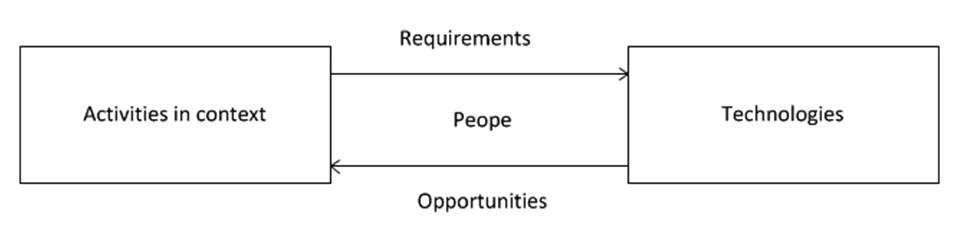
\includegraphics[width=0.70\textwidth]{img/PACT.png}
	\caption{PACT model}
	\label{fig:PACT}
\end{figure}



\subsubsection{People - the kindergarten teacher}
Kristine is in her thirties and is a fully educated pedagogue. Beyond this she has taken several degrees and courses focusing on the needs of children with mental handicaps, all resulting in her now working at Birken.

She takes care of a select few children of those attached to the kindergarten, an activity that requires almost constant supervision while they are present. Kristine and her colleagues yearn for solutions that can ease and improve their daily work, particularly within the domains of communication with the children and their parents. Very notably, the time required to add a picture to an entry in the child's contact book is so severe that she cannot do it very often, a hindrance that bothers her. She would very much like to be able to attach an image to the book every day to improve the dialogue between child and parent.

\subsubsection{Activities}
\begin{itemize}
	\item Each day an entry is written in the contact book of every child, detailing the highlights of the day. It may be a single sentence or a paragraph with a picture of the child engaging in an activity. This is done by the guardians at the kindergarten, but entries may be commented or entered a new by parents with any important thoughts.
	\item If a picture is to be added, first the picture is taken with a digital camera, imported into a desktop computer, then cropped, resized or rotated as necessary. Finally, the image is printed onto paper, cut out and glued into the contact book.
	\item Child and parent will sit down with the book, using the image in the book (if present) as a starting point for dialogue about the day, continuing through available pictograms.
\end{itemize}

\subsubsection{Contexts}
There are three contexts based on the three activities, two of them sufficiently similar to be written as one.
\begin{itemize}
	\item When compiling an entry in the contact book, the kindergarten teacher or guardian will sit by themselves, the child occupied either with their own devices or the supervision of someone else. 
	\item When discussing the entry in the book, however, child and parent are together.
\end{itemize}

\subsubsection{Technology}
Currently, two hardware technologies are in play: A digital camera, and a personal computer.
An image manipulation suite is used to edit the photographs. Possibly, this is a Windows pre-installed application like MS Paint.

\subsubsection{Conclusion}
Even at a glance, several possible improvements can be suggested that make use of IT. Central are the notions of digitizing the contact book and easing the creating of images by using a mobile device with image manipulation software capable of the actions usually necessary.
\section{Illustration of the system}
The idea with making a rich picture is to get an understanding about the current interaction with technology. This is an overview of how the users who are the guardian and pedagogue and the child would interact with the mobile device. Under the assumption that the multi-bachelor project has been implemented in the everyday life to show how it could be improved with an administrator program on the computer.

In the current system the administrator who has the task of administrating the setting, program and data on the mobile device, now also has to be done on the mobile device. At the same time the child also have tasks on the mobile device which then create a problem between child and administrator when they need the mobile device at the same time. The mobile device is used by the child as a communication tool so the administrators are able to understand what the child wants or needs. Though this understanding the child and administrator can easier communicate in their everyday life.

The current problem with the mobile device is that both the administrator and child need it and some children would consider the mobile device theirs and therefore wound not hand it over to the administrator. To resolve this problem and computer program could be made from where the administrator could change the setting and data which then via Wireless Internet and a server then could administrate the mobile device. This picture is shown in \vref{fig:Rig billede}. 

\begin{figure}[ht]
	\centering
		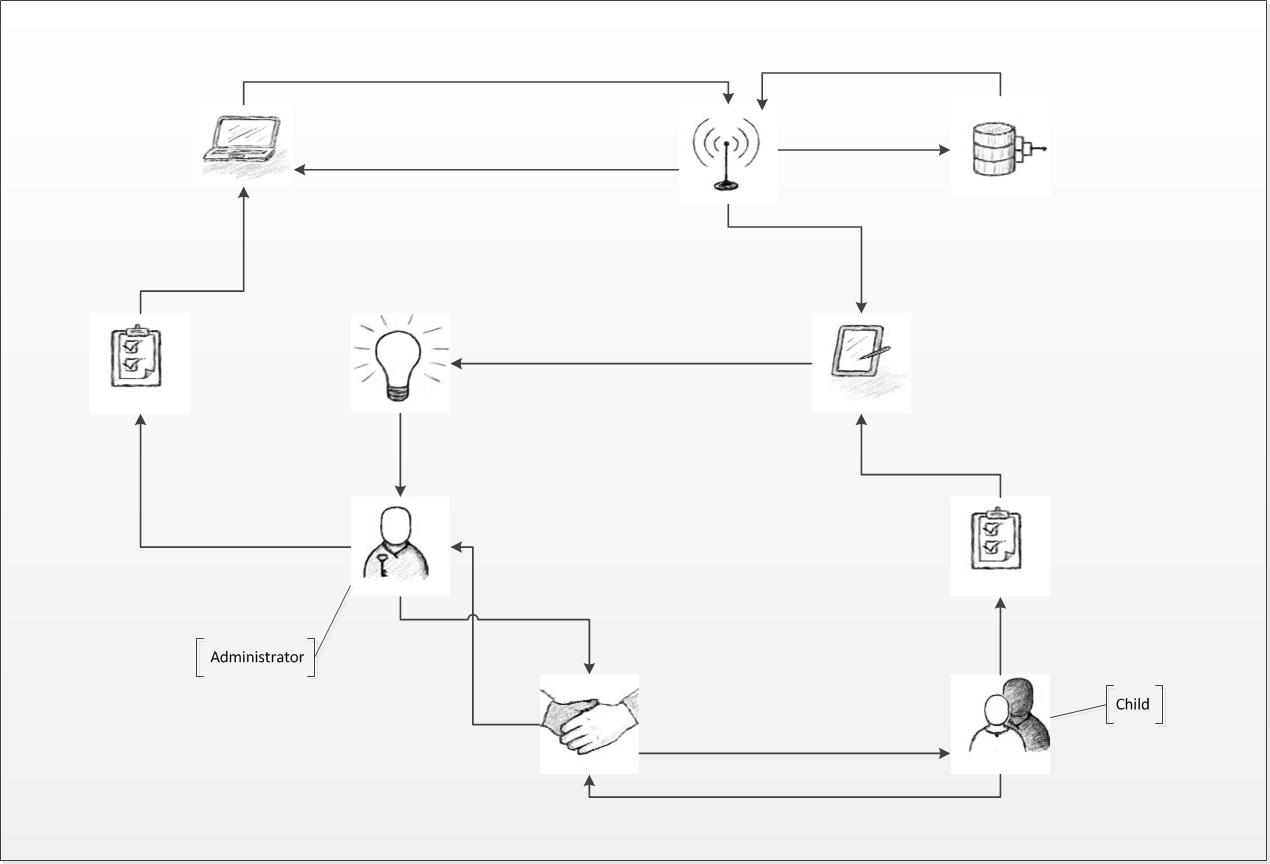
\includegraphics[width=1.00\textwidth]{img/Rig_billede.jpg}
	\caption{How the solutions should be}
	\label{fig:Rig billede}
\end{figure}

In our project we also want to make a digitized version of the contact book such that the guardian and parents easily and quickly can send small messages to each other. Furthermore the guardians would be able to send a summary of what the child have been doing today and include pictures of the child doing an activity. This is the base for our system definition.    

% kapitel systemdefinition
\chapter{System definition}

\section{BATOFF}
This is a BATOFF analysis of the online journal for parents and pedagogues to communicate in the everyday life. The journal should be available from the tablet such that a pedagogue can snap a picture, write a post and upload it for the kindergarten teacher or guardian to read. BATOFF is a tool to define a product.

\subsection{Betingelser - Conditions}
There are several requirements for the journal to work:
\begin{itemize}
	\item There has to be a connection between the mobile devices, such as the tablets, and the platform. 
	\item It should be easily accessed by people with little IT-experience, as we have very little knowledge about the users, especially the parents.
\end{itemize}

\subsection{Anvendelsesomr�de - Scope}
The scope for the journal concerns the pedagogues, parents and guardians and in some regards the autistic children. Furthermore there will be some administrators maintaining the system:
\begin{itemize}
	\item The pedagogue is a main user of the journal as he or she mostly fills out the journal. The pedagogue should have access to the different children's journal and can upload and edit pictures to add to the journal.
	\item The kindergarten teacher or guardian should only be able to read the journal of their own child, but can edit and add pictures.
	\item The child can read and show their parent etc. the pictures in the journal, but are unable to edit the journal.
\end{itemize}

\subsection{Teknologi - Technology}
There are a couple of technological requirements for the journal to work:
\begin{itemize}
	\item	The platform should be supported by both mobile devices as well as stationary devices.
	\item A database to store information, such as user credentials.
  \item A specially designed framework to handle the journal application.
	\end{itemize}

\subsection{Objekter - Objects}
The main objects for the journal consist of these:
\begin{itemize}
	\item	Mobile devices i.e. the tablet.
	\item	The autistic child as they can read the journal.
	\item	Pictures that pedagogues can take for the journal. 
	\item	The parents/guardians and the pedagogues as the journal serves as a communication between the two. 
	\item	A day, as the journal is most likely edited from day to day and does not matter from i.e. week to week.
\end{itemize}

\subsection{Funktioner - Functions}
The journal itself has a number of functions:
\begin{itemize}
	\item	Write a post of the day for the parents or guardians to read.
	\item	It should be available for both pedagogues and parents to edit and delete posts. 
	\item	Take, upload and edit pictures for the journal. Furthermore pictures should be able to be attached to the post of the day.
	\item	The picture editor should include crop, resize and rotate.
	\item	It should be possible to upload posts from both the mobile device and the stationary.
	\item	(It should be possible for users to see other authorized users.)
\end{itemize}

\subsection{Filosofi - Philosophy} 
The main idea behind this journal is to:
\begin{itemize}
	\item	Aid to the completion of writing and adding pictures to posts.
	\item	Give an administrative tool to manage the journal.
	\item	Improve the communication between pedagogue and parent and the communication between the parent and the child.
\end{itemize}

\section{System definition}
This piece of software is primarily a communication enhancing tool for the guardians and pedagogue for the daily use and secondly a conversation starter with the child. It should be able to send a story/text and pictures back and forwards between the guardians and pedagogue. This should be done by a platform which is supported both on mobile devices and stationary devices.


% 2. Teori om program
\part{Design}
%kapitel OOAskal have klassediagram OOA
\chapter{Analysis of the program}
\section{Modeling of Giraf administration}
To model the Giraf administration program a class diagram was made, see Figure \vref{fig:classOversigt}. This give an overview of what we would have to implement in our program and the class diagram describe, how the base model would look like. The Giraf administration needs a user before it can get all the Giraf administration applications that the user can administer. In the model three different persons is important to remember the child and the users who can be either a parent or a kindergarten teacher. The user needs to have a connection with a child and the child's mobile device before the Giraf administration can detect which Giraf mobile applications the device has and then foreach Giraf mobile application finds the Giraf application administrator. The difference on the two Giraf administration applications is that the Giraf application administrator would have a connection to the application on a device e.g. DigiPECS or aSchedule, while User application only is accessible in the Giraf administration.

\begin{figure}[ht]
	\centering
		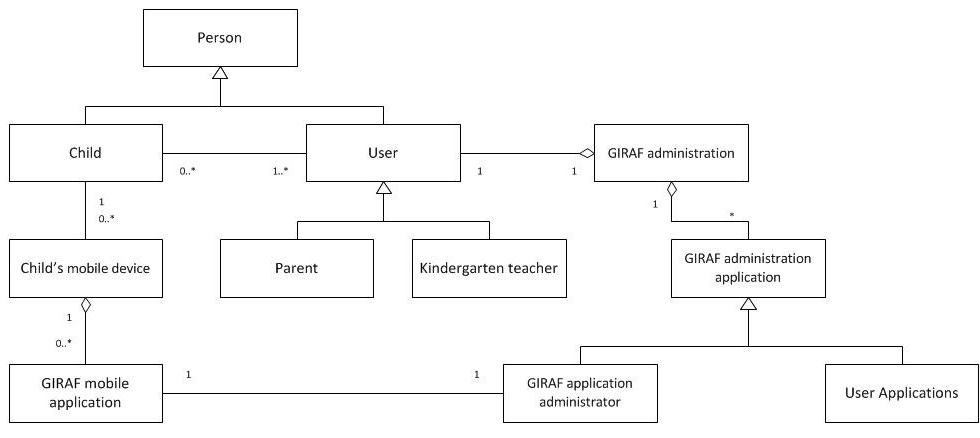
\includegraphics[width=1.00\textwidth]{img/classOversigt.jpg}
	\caption{Giraf administration program}
	\label{fig:classOversigt}
\end{figure}

\section{UI functions}

Function types:
\begin{itemize}
\item{Update: Functions of this type are activated by an event in the problem area. Result: state-change in the model.}

\item{Signaling: Functions of this type are activated by state-change in the model, resulting in reaction in surroundings. Reaction can be a presentation for the users involved in the scope or direct intervention in the problem area.}

\item{Readings: Functions of this type are activated by the need of information in a user's tasks. Result: system displays relevant parts of the model.}

\item{Calculation: Functions of this type are activated by the need of information in a user's tasks, consisting of a calculation, which involves information from the user and the model. Result: Displaying the result of the calculation.}

\end{itemize}

The simple, medium, complex tags indicate how simple or complex the functions are to implement according to the development group.

\begin{table}[!ht]
\centering
\begin{tabular}{ l  c  c }

Login Screen: &  & \\ \hline
login & Simple & Update \\ \hline
forgotPassword & Simple & Update \\ \hline
register & Medium & Update \\ \hline
\end{tabular}
\caption{Login screen functions}
\label{tbl:loginscreen}
\end{table}

\begin{table}[!ht]
\centering
\begin{tabular}{ l  c  c }

Newsfeed: & & \\ \hline
getNews & Simple & Readings \\ \hline
addNewsPost & Medium & Update \\ \hline
canUserPost & Simple & Signaling \\ \hline

\end{tabular}
\caption{News functions}
\label{tbl:newsfeed}
\end{table}

\begin{table}[!ht]
\centering
\begin{tabular}{ l  c  c }

Main menu: & & \\ \hline
signOut & Simple & Update \\ \hline
getMyAccount & Simple & Readings \\ \hline
getGroup & Medium & Update \\ \hline
getGroups & Medium & Readings \\ \hline
getChildList & Simple & Signaling \\ \hline
getAppList & Simple & Signaling \\ \hline
setView & Complex & Readings \\ \hline

\end{tabular}
\caption{Main menu functions}
\label{tbl:mainmenu}
\end{table}

\begin{table}[!ht]
\centering
\begin{tabular}{ l  c  c }

Contacts: & & \\ \hline
getMessage & Medium & Readings \\ \hline
getMessageList & Medium & Readings \\ \hline
addNewMessage & Medium & Update \\ \hline
getCurrentUser & Simple & Readings \\ \hline
uploadImage & Medium & Update \\ \hline
addNewReply & Medium & Update \\ \hline

\end{tabular}
\caption{Contact book functions}
\label{tbl:contactbook}
\end{table}


%kapitel med design OOD
\chapter{Design}
\input{tex/componentarchitecture.tex}
\section{Prototypes}
There were used different prototypes to decide, how this program should interact with the user and how the user interface should look like in the end. In this section three different prototypes will be shown and the work process and decision making will be explained.
The first prototypes were drawings on a blackboard or a piece of paper but later we also had an HTML prototype. In this process 2-3 group members made the first design and the presented it to the group which when came with point of improvements which then was discussed and then a new prototype was made until the design was satisfactory. The HTML prototype was also shown to the kindergarten teacher Kristine in the second interview which has summarized in \vret{firstInterviewBirken2}.

\subsection{The first prototypes}
After the first prototype was presented each page was drawn on to the blackboard where the changes easier were added. One of the first blackboard designs of the page change settings of a child which is e.g. the child's name and abilities is shown in Figure \vref{fig:firstProto}. This is a primitive design with two menus one horizontal and one vertical, where the horizontal has all children and groups of children and the vertical has all the applications on a child's device the user can administer. This menu will be further explained for the next prototype. 

\begin{figure}[ht]
	\centering
		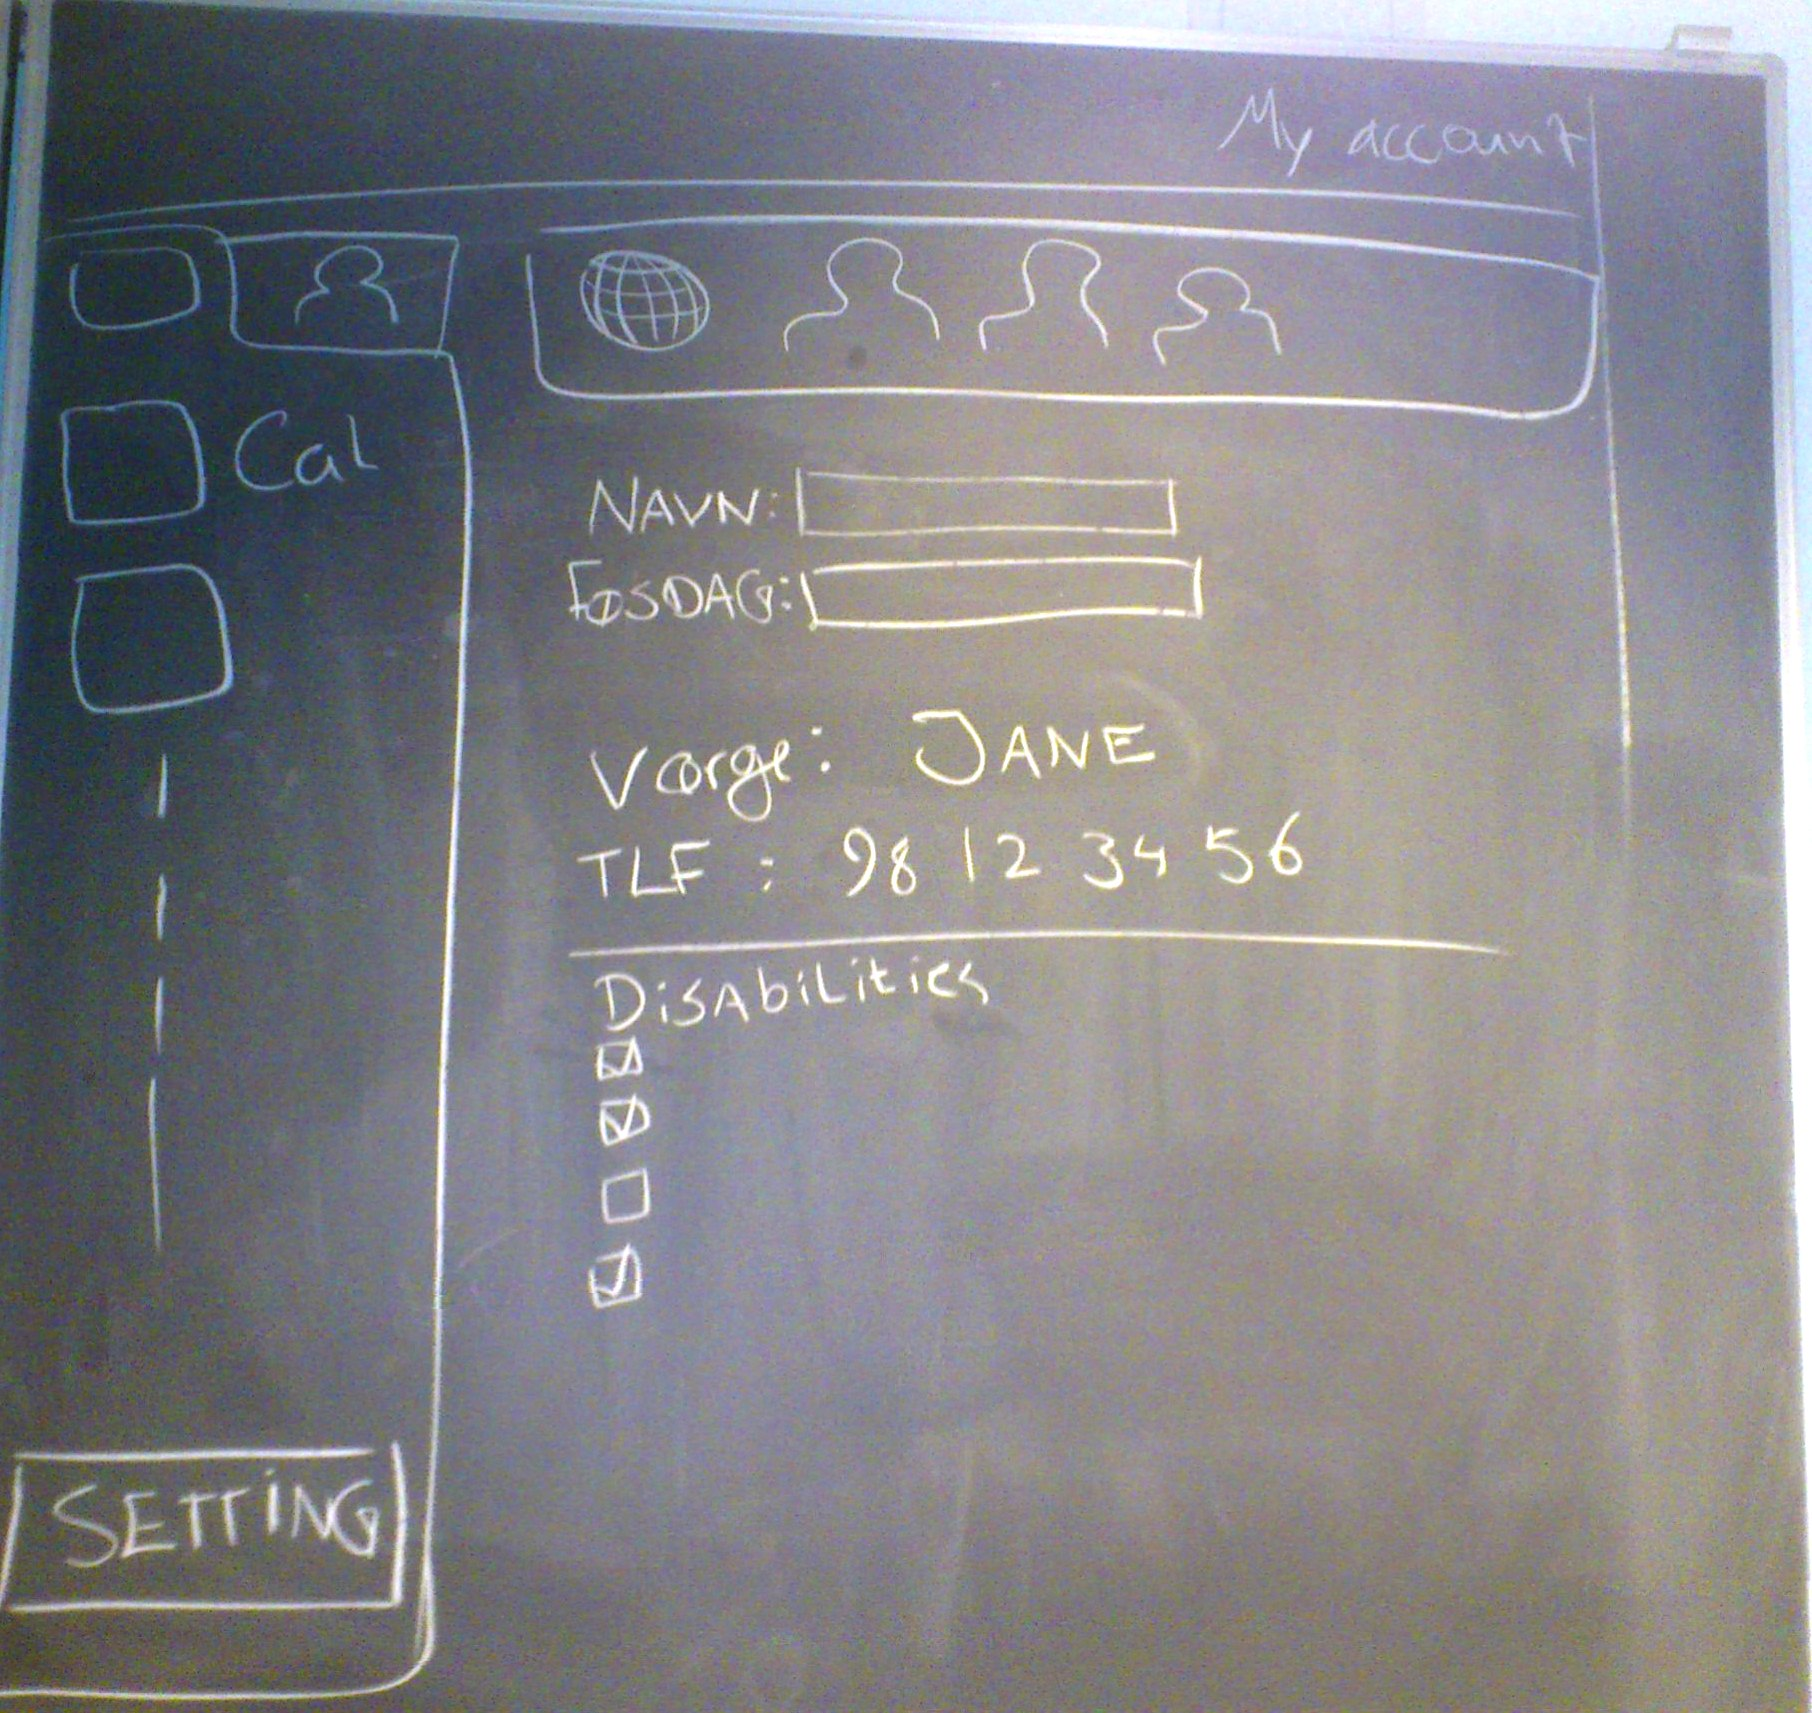
\includegraphics[width=1.00\textwidth]{img/firstproto.jpg}
	\caption{?Changes made on the black board?}
	\label{fig:firstProto}
\end{figure}


The group members did disagree how to get into this page, because in this design the user would have to choose a child in the top horizontal menu and the press the Setting button in the vertical menu, which is located among Giraf application that is to be administrator. Especially the location and the naming of the Setting button were discussed because the user would get the impression that they administer their child like the applications and not changes the information about the child. To solve this it was suggested that this page should be in My Account instead; where the user also would be able to change they own personal information. In our prototypes this was not change until the implementation. ?????not sure????% sp�rg johannes eller se n�r den er f�rdig

\subsection{The HTML prototype}
For the second interview with Kristine an HTML prototype was made from the primitive prototypes. The Figure \vref{fig:contactbook} is two screen shoots from the child Jack's contact book where the right side of the figure is an Light box with an entry from the contact book. The contact book is inspired by a calendar, because for a date it can have some entries that the user can click on and then within a Light box the message and pictures is shown. If the user has not seen the message before, the signal "Ny!" in the right side should be visible. The user is able to fold and unfold the entries for each date, to see or hide the entries in the contact book. 

\begin{figure}[ht]
	\centering
		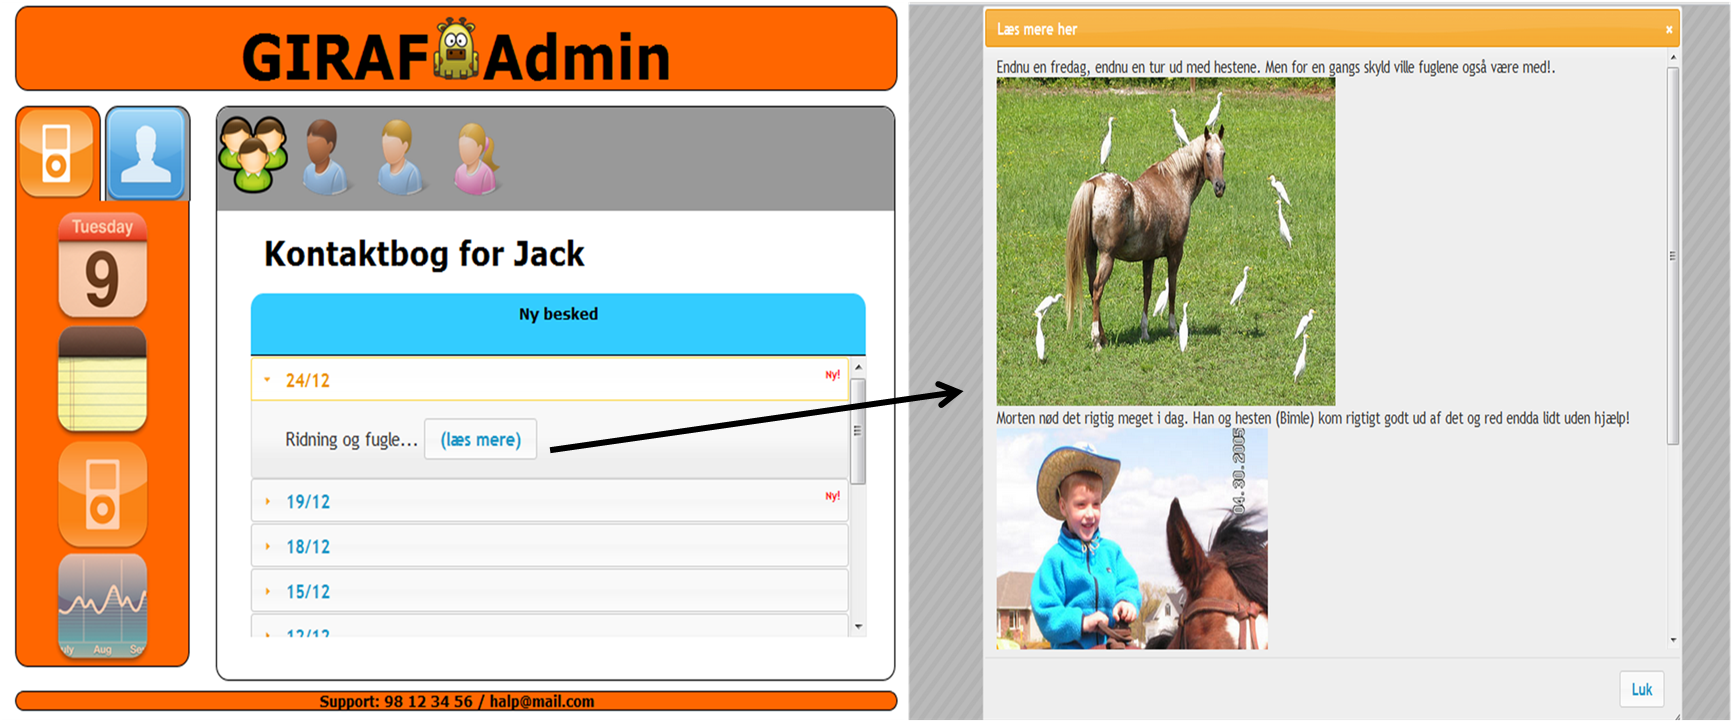
\includegraphics[width=1.00\textwidth]{img/contactbook.png}
	\caption{screenshots from the html prototype}
	\label{fig:contactbook}
\end{figure}

\subsubsection{The menus}
As shown in Figure \vref{fig:contactbook} the Giraf applications' administrators is represented on the vertical menu, as an icon that should identify the application administrator. The children's devices are represented on the horizontal menu where the single child's device is identified from a picture and the group is identified by an icon representing a group of children. However this representation can be mirrored such that the children's devices are represented on the vertical menu and the applications are represented on the horizontal menu, which is shown in Figure \vref{fig:menus}. The black circle indicates which of the menus is represented in the vertical menu. This menu was not implemented because it would take too much of the space on the screen, and it could also be a confusing navigation path for the user, without gaining any new functionality. In the next paper prototype this menu was replaced with two vertical menus side by side.

\begin{figure}[ht]
	\centering
		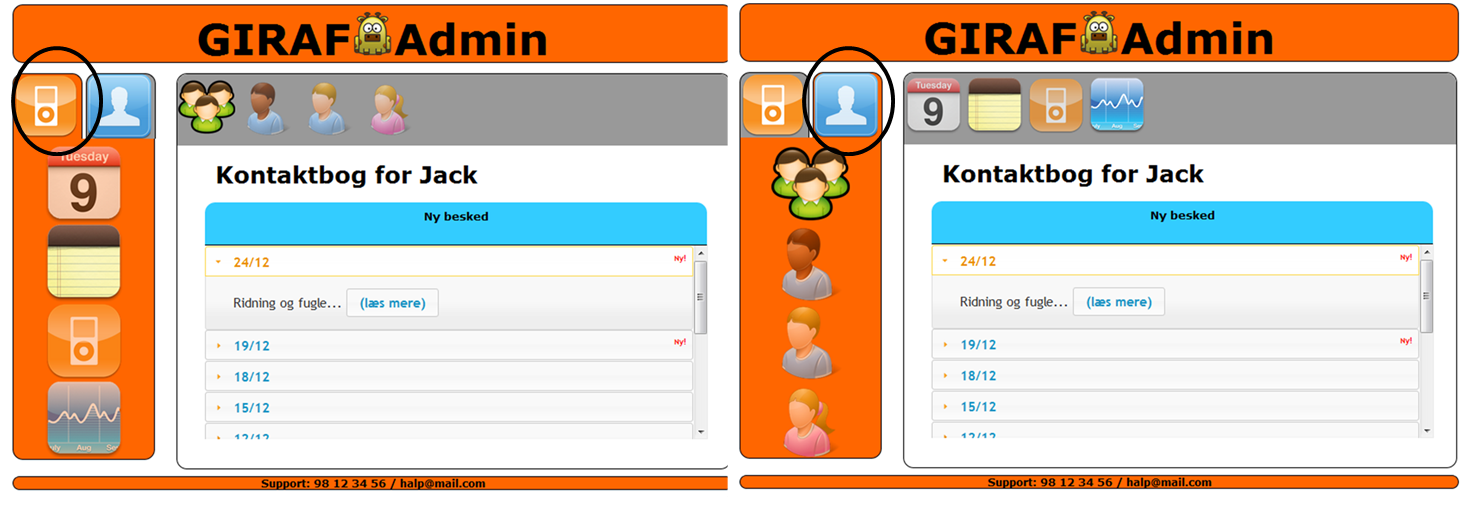
\includegraphics[width=1.00\textwidth]{img/menus.png}
	\caption{The prototype menus }
	\label{fig:menus}
\end{figure}


\subsubsection{Evaluation of the HTML prototype}
In the second interview in \vref{firstInterviewBirken2} with Kristine from Birken we introduced the HTML prototype to her. In general she thought that it was a nice design and she commented that the icon for a child should be a photo of the child instead, which also was indented. She also missed a way to make a reply to a message which would be useful since it is used both by the parents and kindergarten teachers. Kristine said: "[communication] \textit{It goes in both directions. The parents write in the contact book in the morning and we write during the afternoon which then can result in a longer dialog between the parties.}" from the interview in \vref{firstInterviewBirken2}. The reply function was then included during the implementation. 

She tried to create a new massage and wondered if there was a spelling checker, that would detect misspellings and she would like there to be one. However, we think this to be a minor issue that could be implemented later. 

She saw two versions of the contact book the first could have several pictures and text while the other had some text and only one picture was the message see Figure \vref{fig:createmessage}. She said: "\textit{both can work - because what we do when we are on a trip and add pictures is that we always write something to the picture, but also some general information about the day's events. ... What I think that you somehow can separate the text}" from the interview in \vref{firstInterviewBirken2}. This functionality was added in the contact book during implementation, where each picture can have some text add with it and a text field for the general information about the day. 

\begin{figure}[ht]
	\centering
		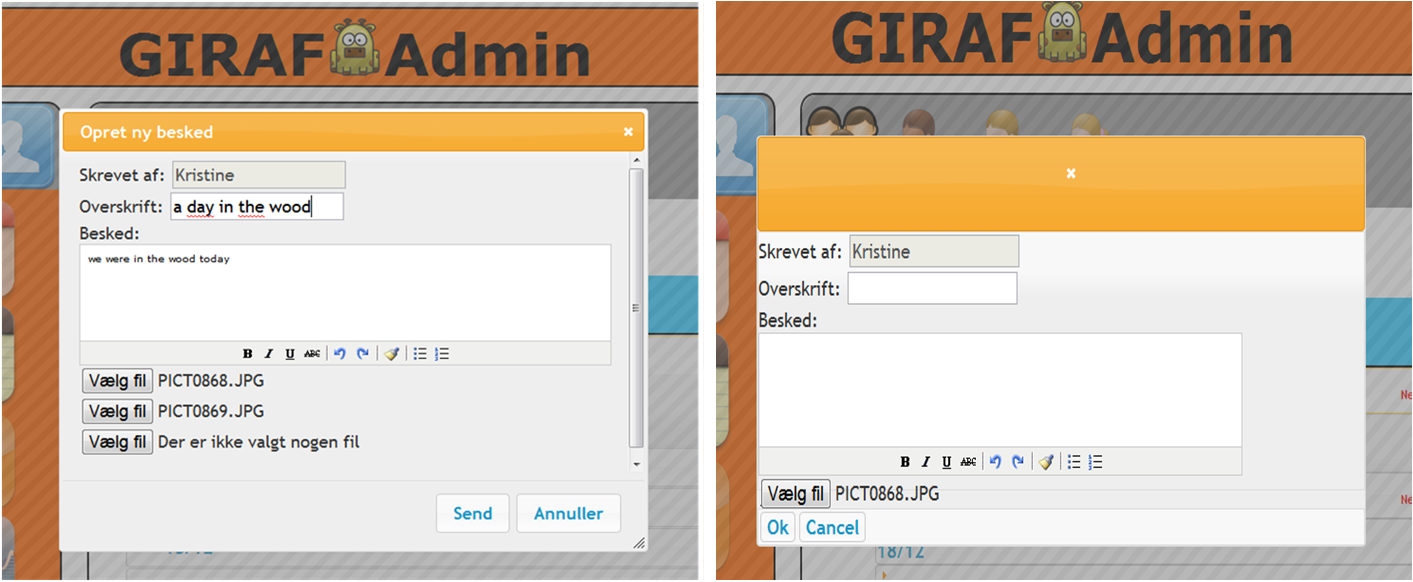
\includegraphics[width=1.00\textwidth]{img/createmessage.png}
	\caption{create message}
	\label{fig:createmessage}
\end{figure}

In the beginning of the interview she showed us a standard information sheet that contained the child's name, the parents' name and contact information. The current contact book has this sheet in the first page and Kristine though that it also should be included in the digital contact book. However, the sheet will not be placed with the contact book, and she suggested that a button among the other applications' administrators like the Settings button from the first prototype. But we would rather place the information with the other information about the child. 

During the interview expressed that they rarely did edit pictures before printing, but if they were to upload a picture in a message and easily had access to quick rotation, crop, enlarge/reduce size of the picture then she would probably use it, however, then she would also need an undo button. These functions would be nice to have, but it would not be a priority to be implemented.
From our prototype it was not clear that it would be a closed system, where the kindergarten teachers and parents would have to login before they would be able see or write in the contact book. She thought this very important because the information in the contact book is very sensitive information and the personal Data Protection Act%(persondataloven?)
 covers this area. 

Kristine pointed that now when a child moves on from the kindergarten the child always gets all of his/hers the contact books. If this digital contact book were used instead this tradition would be lost, therefore she suggested that the user e.g. were able to print the contact book so it was not lost afterwards since Birken are not allowed to have these information indefinitely because of the personal Data Protection Act. The solution to this problem should then be studied further.

After the interview we also wanted to have a start page with general information about the meetings and news from Birken to the parents. Kristine first talked about this information in relation to the calendar which only is represented by an icon in the prototype, but that calendar was only supposed as the child's calendar so the other solution was preferred.

\subsection{The last paper prototype}
In the last primitive paper prototype of the design the menu has change to two vertical menu, where the user need to click on an application, a child and then press a go-button to get the application for a or all children. This is shown in the Figure \vref{fig:calendar} in which the application aSchedule's administrator for Jack is called, however we never implemented an administrator module for aSchedule. When this design was evaluated we thought it would be easier to understand and implement if the user should choose a child or a group of children first and then choose an application, because the applications' administrator depends on the installed applications on the child's device. The go-button was not necessary and was abandoned, while the button Settings was also abandoned as mentioned earlier.

\begin{figure}[ht]
	\centering
		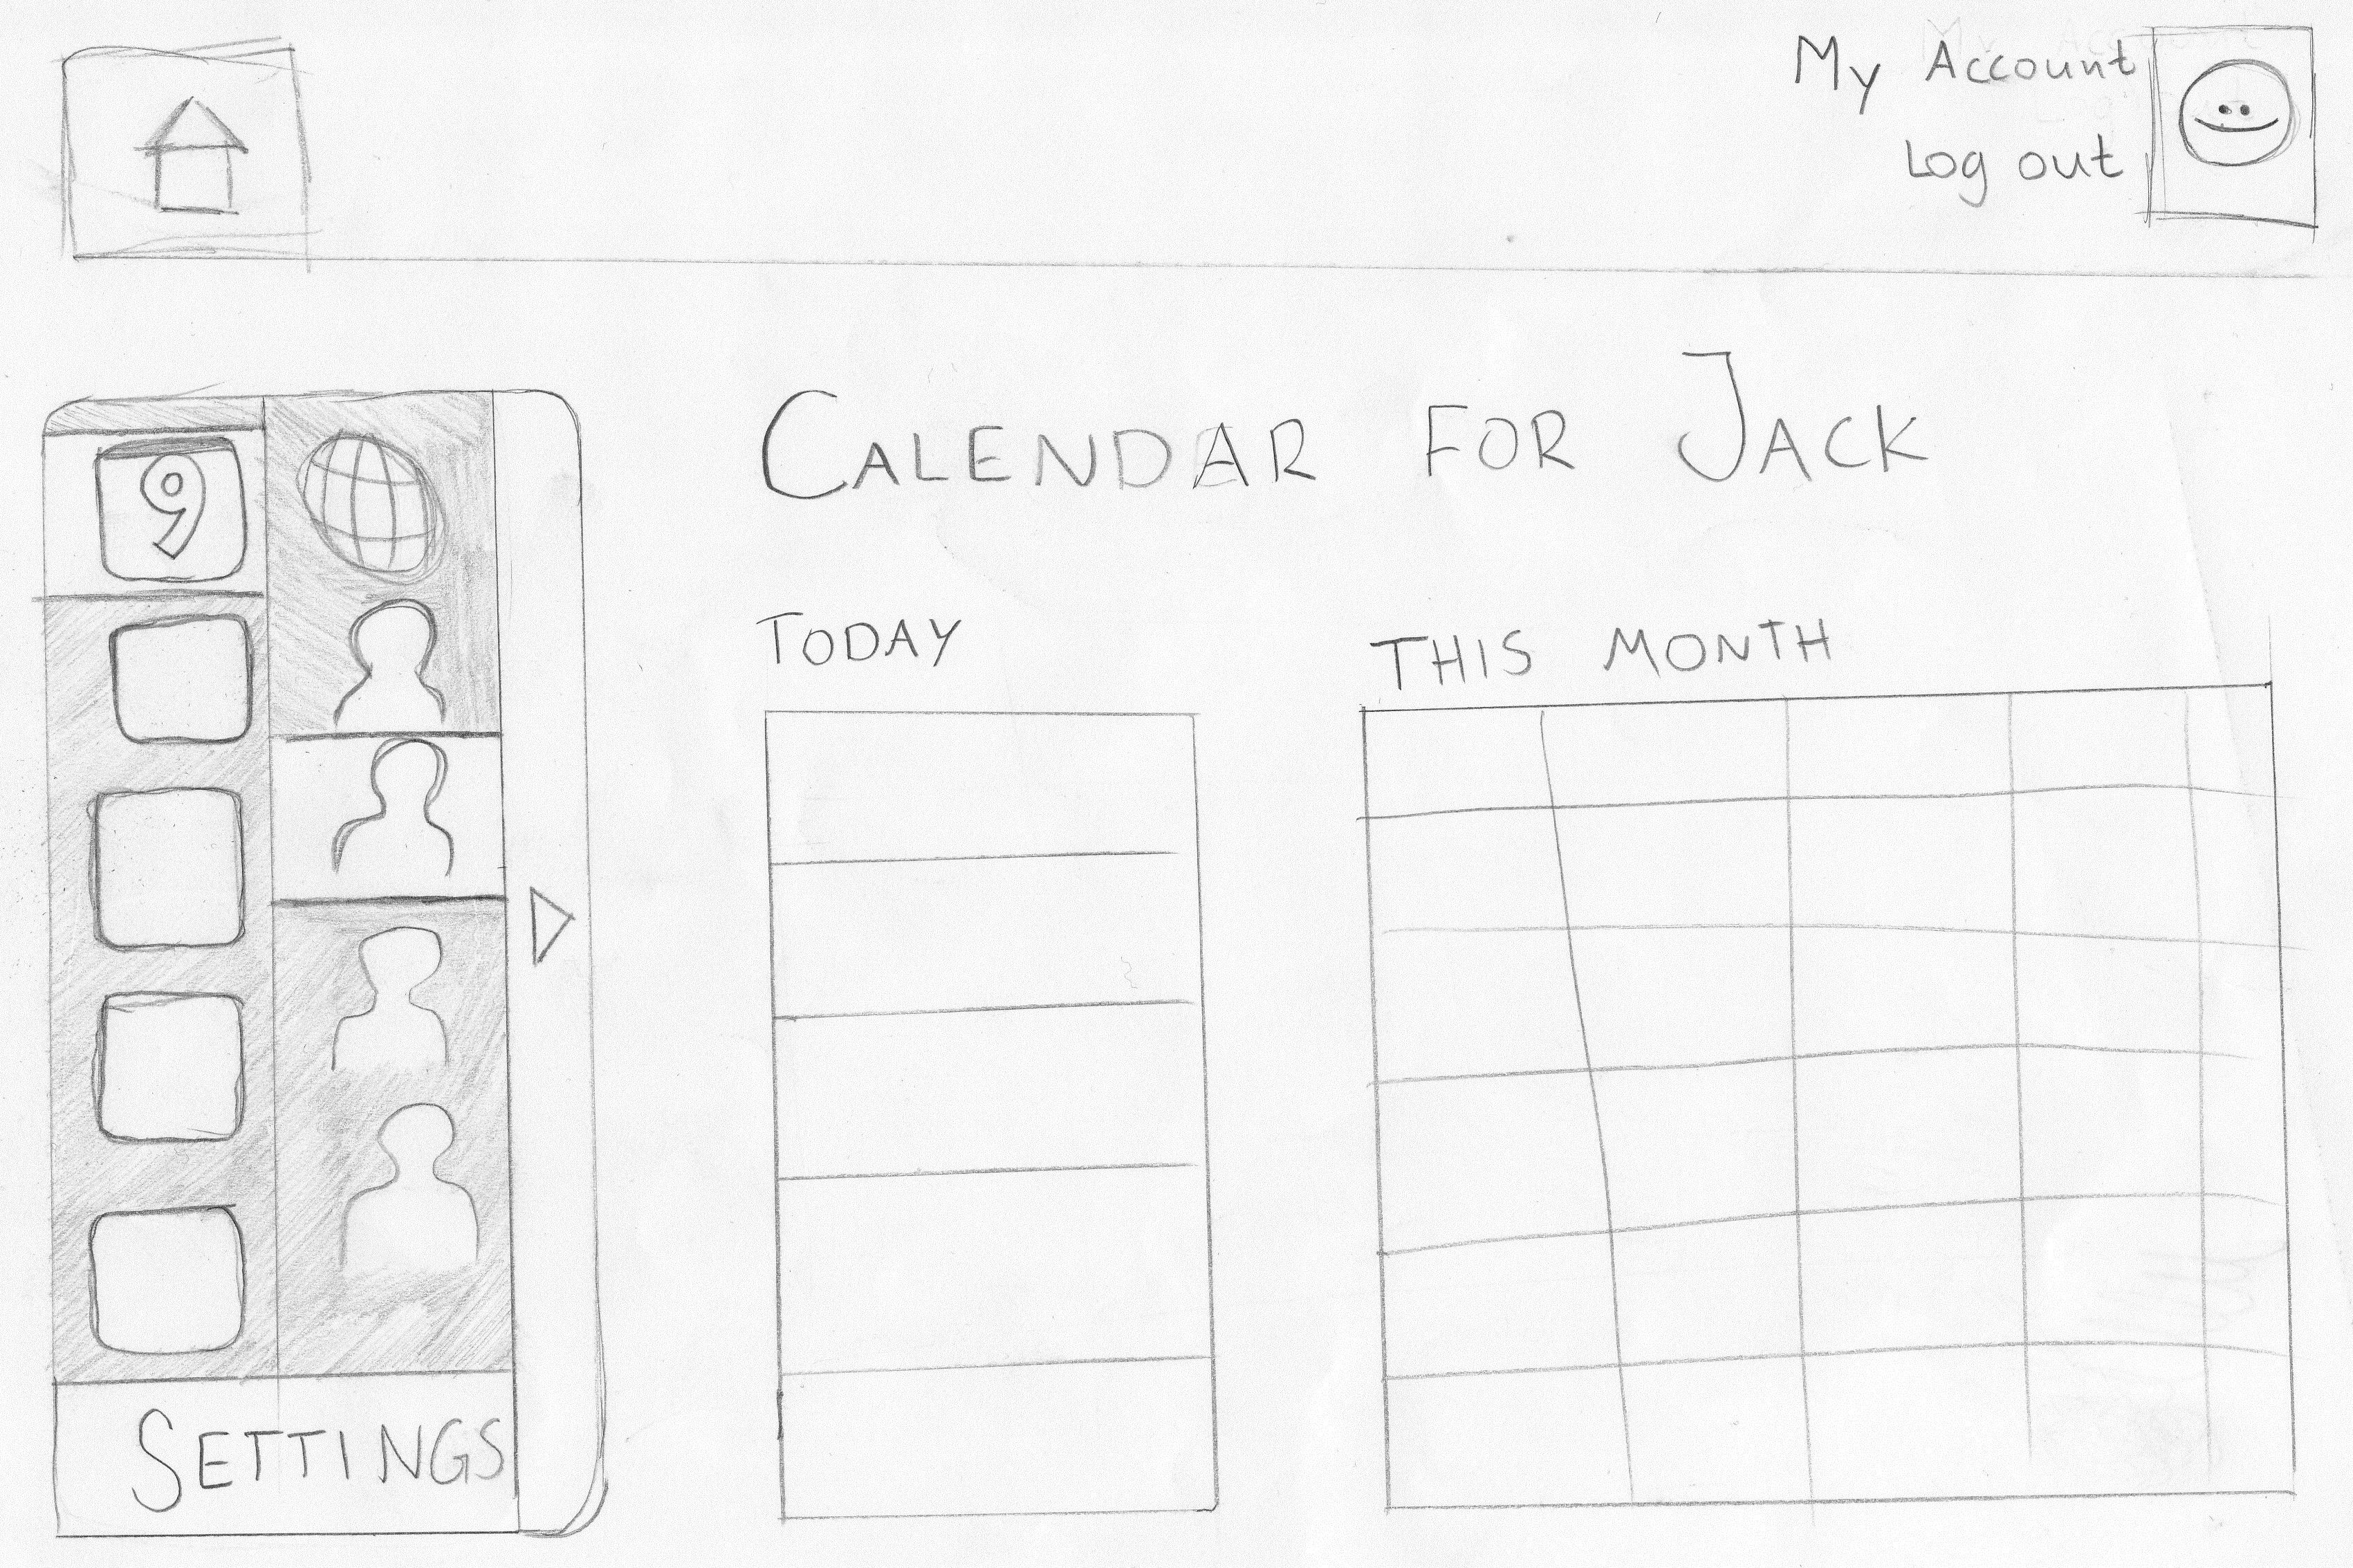
\includegraphics[width=1.00\textwidth]{img/calendar.jpg}
	\caption{calendar}
	\label{fig:calendar}
\end{figure}

  
In the top-left corner of the prototype is the homepage button which page should contain general information and news from the kindergarten, this was one of the changes made as a result of the interview with Kristine. In the top-right corner should be a logout button and My Account button, which leads to the personal information that is show in Figure \vref{fig:myAccount}. 
\begin{figure}[ht]
	\centering
		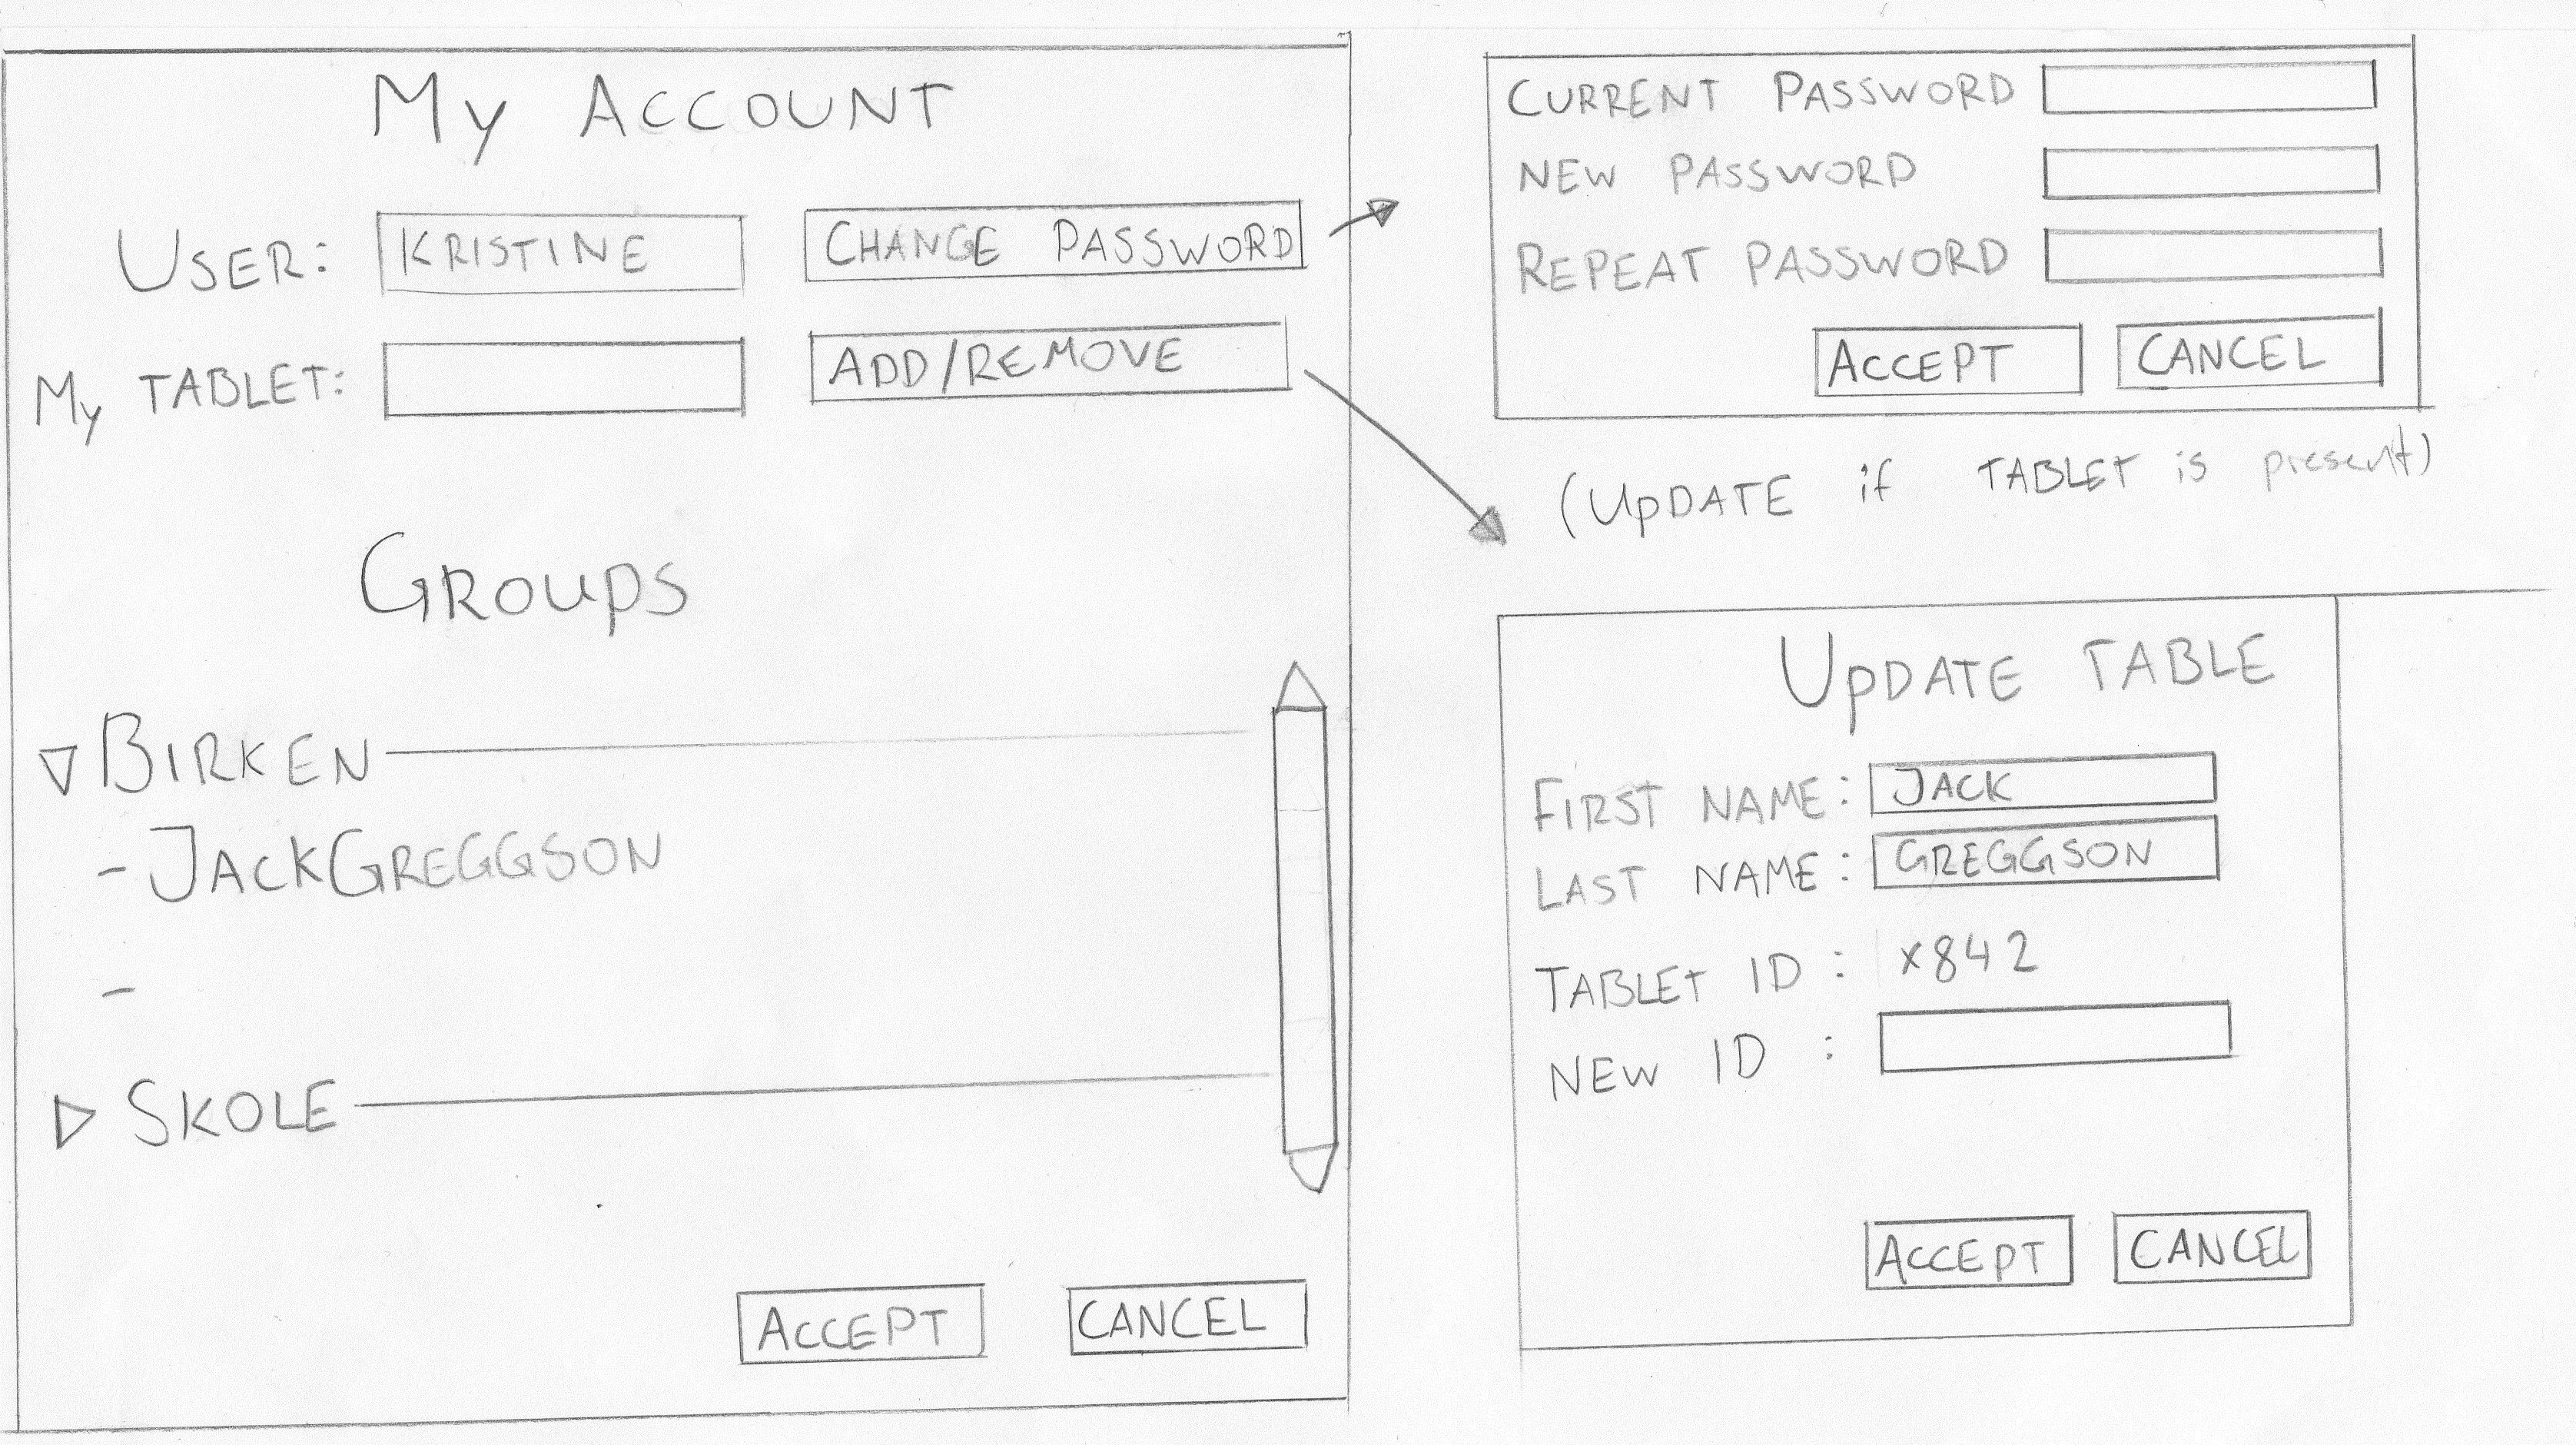
\includegraphics[width=1.00\textwidth]{img/myAccount.jpg}
	\caption{Design of My Account}
	\label{fig:myAccount}
\end{figure}


In this prototype design there are only one page and two pop up boxes, in the first can the user change his/hers password and in the other the user can add/update or delete a device. On the My Account page the user could also see or update devices in a group, however, this design is confusing. This design was not thought through because the field My Tablet could be the users own mobile device, and in the beginning it was meant as his/hers child's mobile device and in both cases the user could have more than one mobile devices that should be registered but cannot in this design. 

The group under My Account is needed, because the user of this administration program could both have access to use this tool privately and work-related, such that the user is parent to an autistic child and is also kindergarten teacher for some other autistic children. This mean groups would be necessary when the user wants to change something on all but his/hers child's device without repeating the same process on all the other children's' devices. The design missing something that indicates, how the user can add a device to a group. In the evaluation of this prototype it was also decided that My Account also should contain the child's personal information and device. In the implementation it was also decided that user information, group and child plus child's device should be under different tabs.   
 





% 3. Implemetation
\part{Implementation}
\todo{Still to be planned}
%
\part{Evaluation of the program}
\chapter{Theory}

\section{Usability}
When developing software and other products that require user interaction, one must be aware of the usability of the product and how to evaluate it.
Usability is a quality attribute, which is fundamental to a successful product and is defined by 5 quality components:
\begin{itemize}
	\item Learning: How easy is it for users to accomplish tasks during first encounter of the design. 
	\item Efficiency: After learning how the product works, how fast can they perform various tasks.
	\item Memorability: After a period of not using a product, how easily can they obtain efficiency again.
	\item Errors: How many errors do users make and how easily can they recover from the errors.
	\item Satisfaction: How pleasant is it to use the product.
\end{itemize}

To explain the importance of usability and how it is fundamental to a successful product, one must understand that no matter how a product functions, as long as user interaction is required, it must comply with the needs of the user and help to complete the tasks at hand.
As an example one can look at a website. If a website is difficult to use, if users get lost trying to browse the website or the information stored on the website is hard to read and/or figure out, people tend to look for alternatives. This results in loss of customers and therefore is bad for the company that designs, hosts and administrates the website.
If a product on the other hand is designed for a special purpose where no alternatives are to be found, like a system to administrate a hospital. Usability is so important that errors could lead to serious harm of patients. Reasons can be efficiency or errors, where time spent figuring out the system means delay in service and errors can result in system stalling or misinformation.

There are methods for studying and improving usability but user testing has proven the most useful and will therefore be the project�s focus when evaluating usability of the product.\cite{usability} %skal evt flyttes til evalution
\todo{Still to be planned}

\part{Conclusion}
\todo{Still to be planned}

\addcontentsline{toc}{part}{Listings}
\listoffigures
\lstlistoflistings
\label{lastpage}

% Change headings for bibliography. Looks fucked otherwise, I think.
% Page design from fancyhdr.
\fancyhead{}
\fancyfoot{}
\fancyhead[RO,LE]{\leftmark}
\fancyfoot[C]{\thepage}
\setlength{\headheight}{23pt}

% Afslut med bibliografien

\cleardoublepage
\phantomsection
\addcontentsline{toc}{part}{Bibliography}
\bibliography{bib/bibliografi}

% 4. Bilag
\appendix{}
\addcontentsline{toc}{part}{Appendix}
\chapter{Interviews}
\section{First meeting with Birken}
\subsection{Disposition}
\begin{itemize}
	\item Avoid boolean or leading questions.
	\item Scenarios:
		\begin{itemize}
			\item digiPECS
			\item aSchedule
			\item plAytime (displays play instructions)
		\end{itemize}
	\item How could you administrate devices/applications? Suggestions?
	\item Rich pictures/images
	\item How do you create new or better meanings in communication?
	\item Prototypes
	\item Clear usage of time.
		\begin{itemize}
			\item Right now, what do the parents do, what do you do? (Explorative)
			\item Do you regularly discuss the child and their activities? How do you communicate? (Verification)
			\item Do you make detailed scheduling? Are the children involved in this activity? (Verification)
			\item How does a usual day play out? (Explorative)
			\item How do you communicate with the children? (Explorative)
			\item Reaction on removing their items (like a phone)? (Verification)
		\end{itemize}
\end{itemize}
\subsection{Questions proper}
\begin{description}
	\item[10 mins] Introduction (names, the group, overall project goals, our intentions with the meetings)
	\item[10 mins] Introduction of the currently working GIRAF system, excluding the admin app - this is done specifically to avoid associations with that app when IT options are discussed.
	\item[5 min] Our specific goal, a PC-based administration program.
	\item[20 min] How is a typical day (or week) structured for the supervisors?
		\begin{itemize}
			\item Areas of responsibility (parents vs. supervisors)
			\item How is planning done? During the work day and how far ahead?
			\item Does the institution have access to a PC?
			\item Variation in daily activities.
			\item Is it a realistic goal to give children access to a tablet? In an estimate, how large a group of the children are functioning high enough to work with such a device?
		\end{itemize}
	\item[20 min] Communication
		\begin{itemize}
			\item Which methods of communication exist for children with autism beyond imagery/pictograms?
			\item How is a single day's schedule presented? One event at a time or a large presentation at the beginning?
			\item How are new meanings introduced to non-verbal children? For example new pictograms.
			\item Are the children involved in deciding the activities?
			\item What kind of reactions could be expected from removing an item they consider theirs?
		\end{itemize}
	\item[25 min] abstraction to IT solutions
		\begin{itemize}
			\item Debate possible IT solutiosn to ease/improve the daily work.
			\item How can It improve your working day?
			\item Optionally consider directly discussing administration solutions or work with rich pictures. Bring blank paper to draw on if possible.
		\end{itemize}
\end{description}
\section{First interview with Birken}


Even before our input there was a clear desire to utilise IT to extend and improve communication by words.

Birken has a single child capable of working with actual words, otherwise the children most effectively communicate using the imagery of pectograms. However, the sounds, names and textual representations are very important in the discourse with guardians. Although a child may only signal a meaning with the image, they respond very strongly (and positively) to a reaction from the guardian if they respond with the word and possibly a complete sentence. While the child cannot speak the word, they can recognize it and the agreement in meaning is essential.

A flexible approach to imagery is very important. Images that most people would immediately understand with an exact meaning can be much more difficult for an autistic child to put into context. As a concrete example, Christine mentions that a child she worked with was unable to comprehend their usual image for washing hands \todo{Get me an image of it.}, instead focusing intently on the head of the tap that to him resembled a power plug. These very particular needs play an important role when the guardians construct imagery via their current solution, Boardmaker, where they are currently forced to take a stock photo, manually (by pixel) delete unwanted parts of the image, and superimpose another to generate the desired result.

\todo{I pushed this a bit in the interview} Just as with anyone else, it is very helpful to know explicitly when a change is made to a known data set. Likewise, the administration module should not aim to create a remote chat feature with the children or changing a schedule without their knowing, but preferably asynchronous planning. What Christine suggested at this point, was to have a default set of daily schedules that could be easily modified for daily use. She mentions that although they work with somewhat static weekly schedules (meal times, for example, or riding every Friday). She confirms that some children have sufficient capacity to memorise their entire daily schedule after seeing it at the start of the day - thus any changes need to be actively communicated to the child.

When asked about the weekly schedule, Christine mentions that from one week to the other, the weeks are somewhat rigid. Particularly when external sources are involved they cannot be debated - this involves riding on Fridays and various health assistants on other days. Changes are allowed if deemed necessary, as well as teaching children the inevitable changes of even the most regular schedule.

A single day:
\begin{description}
	\item[7.30 to 8.50] The children arrive
	\item[9.00] Preparations for breakfast. Toilet visits, diaper changes and most importantly washing hands.
	\item Song.
	\item Variable time - either static weekly event or a choice of several activities, given to the child.
	\item Reading (aloud?).
	\item Washing hands.
	\item Lunch.
	\item Various activities.
	\item Playground time.
	\item Washing hands.
	\item Fruit.
	\item Possibly new diapers, toilet visit.
	\item Taxi cab home.
\end{description}

As Christine puts it, the absolute parts of a schedule are meal times (ALWAYS preceded by washing hands) and song right after breakfast.

(16:00) Upon suggesting that autism causes a very rigid mental model, Christine confirms the almost mechanical precision of regular occurrences. This is however also dependant on taxi cab times.

(17:45) Christine remarks that she has yet to meet a child with autism that knows the meaning of a clock. They use symbols, however, to signal milestones at intervals (for example, they will stick a clear arrow to a point on a clock face to denote where a hand needs to be before an activity ends).

On a peripheral question \todo{Regarding the individuality of grown children}, the general approach used with the children (TEACH) has been in use for at least 10 years. The support of the children continues throughout their education, but Christine emphasizes that she does not know any statistics on how well the children develop later on, remarking that in that regard they are no different from children without autism.

(22:00) Jumping from a reference from Ulrik that the primary method of communication between parents and supervisors happens through the physical contact book that the child brings back and forth every day. When first admitting a child the two parties very specifically, and in great detail, learn about the child and basic likes and dislikes. Direct contact is made when unexpected or somewhat acute events occur, either to discuss or request recommendations on working with the child.

(24:00) On the point of terminology between parents and supervisors, Christine explains that the would mostly be applied in situations where very exact expressions are necessary. Personally, she would use the exact terms and, if necessary, explaining them. As has been noted in other contexts \todo{Document, motherfucker!}, the usage of the exact terminology can seem alienating and create unnecessary complications, as has been the case with immigrants where basic Danish is still an issue.

(27:05) On using terminology in a user interface for parents for a contact book, Christine deflects and specifies that the contact book is also used by the child themselves - most of them understand that it is an extension of themselves. Given daily reports and images of the child during an activity, the parents can use the book as a starting point when reflecting upon the day with their child.

(28:40) Suggesting digitizing the contact book, Christine explains the currently lengthy process of placing images in the contact book. They use digital cameras, importing the images into a computer. Then they crop, resize and rotate the image as necessary (a process she describes as lengthy and hints at usability issues with current applications - in particular she remarks that if the one particular application she prefers to use is unavailable, then she cannot prepare the image), finally printing the modified image and gluing it to the book page.

(29:15) It is very important to Christine and her co-workers to offer the images in order to facilitate communication between parents and children about the past day. Particularly focusing on the child's understanding of imagery, images within the contact book would aid them in reflecting on a situation or experience (while they may only have experienced riding a horse from within "their own head", seeing themselves on the horse from a third person's viewpoint gives greater detail).

(31:20) At this point the mobile device is discussed almost exclusively as a digitalization of the contact book. During idle time (in-between exercises, or when the supervisors need to write down the day's events) they will look in their book. 

(32:45) Discussing if the children could start using the device as an extension of themselves (constantly at hand with imagery), we debate whether they should have it at hand always. Christine sets up a simple rule: when determining what activity is to follow, the schedule is used. During an activity, it should be left alone. 

(34:00) A free thought experiment, we discuss having a sand timer on the device or possibly lock the device during an activity. Such a lock should be immediately switchable but could also see beneficial usage when set for particular children (she mentions some children are capable of understanding the boundaries of staying within a given activity without delving into other things).

(36:30) Alternative methods of communication. Most (if not all) of Birken's children need a structure in discourse. Given autistic childrens' intense focus on imagery, some require that images are not accompanied with sounds.

(37:40) Asking to a combination of autism and blindness, Christine has not encountered the issue (neither in theoretical or real contexts), but suggests the same approach to understanding as with other children - concretes. When teaching new meanings, children are given real versions (or scale models) of the activity or meaning being described (an actual apple or a small toilet), slowly moving to photo-realistic images of the item and finally to simpler drawings and imagery. Simply replacing vision with touch, the same approach is suggested for a blind child.

Christine remarks that while the children have difficulty communicating, it may very well be that they have a very clear internal understanding of contexts and abstraction, but are simply unable to communicate it outwards. 

(40:45) There are no discrete steps applied for the children, but they do discuss a child's physical age with their estimated mental age. Christine notes that they will never use specific terms to describe a child to the parents (cold, neutral language), instead discussing higher level abstractions. \todo{Note that she later brings out TEACH's six phases of understanding.}

(42:55) The children are registered in an electronic patient journal in a centralised system. Given the security criteria and very sensitive nature of the documents, I suggested not considering this a point of interest for the group. It is, however, completely open to the relevant parties (parents, guardians and assigned medical professionals).

(44:20) Christine mentions their own vision. A tablet (a small, thin screen) that can be brought around, but also hung up, and taken home. Drawing inspiration from conventional kindergartens, Christine mentions chat or forum applications that are offered to allow communicate between parents and supervisors.

I reached 46:30 before going cold :)
\section{Second interview with Birken}
\label{InterviewBirken2}

2:30;  om kontaktbogen: oplysningsseddel medbarnet navns og for�ldres navn samt kontakt til for�ldre. Oplysningsseddel b�de for skilte og samboende for�ldre. 

5:23; Afmelding af taxa sker igennem k�rselskontor eller hvis for�ldrene ved barnet ikke kommer et bestemt dato kan de ringe ind til Birken som s� afbestiller taxaen for den/de dag(e)

6:22; f�rst oplysningsseddel og billed af personale i kontaktbogen? P�mindelser?

Fra 8:00  ser Kristine prototypen og for en lille forklaring af prototype. 

11:50; hendes kommentar:Oplagt at have det s�dan her.

12:00; der blev n�vnt at det burde v�re muligt at svare tilbage p� beskeder, det kunne v�re i en lille boks.

12:24; kristine om kommunikation mellem for�ldre og p�dagoger: "det g�r jo begge veje ig�rs, at for�ldrene skriver til os om morgen og vi skriver om eftermiddagen. Ogs� kan det jo s�tte en hel l�ngere dialog igang"

13:08; hun pr�ver at oprette en ny besked og der bliver auto udfylde afsender, alt efter hvem er logget ind.

15:16; Tekst redigering som at g�re en tekst fed, kursiv, understreget eller �ndre farve, bliver ikke brugt nu, og de kunne bruge det men det er ikke vigtigt.

16:15; hendes kommentar: Stave kontrol kunne v�re smart

Ca. fra 17:00 har Kristine set de fleste elementer af programmet og herefter bliver der diskurreret forbedringer og yderligere kommentar til prototypen. 

17:40: Smart med rigtige fotos af b�rnene (i menuen?) og en kontaktside med de generelle informationer

17:56; n�r b�rnene stopper p� Birken for de deres kontaktb�ger som en gave med r�d sl�jfe omkring. Det kommer man til at mangle, hvad skal man g�re med den digitale kontaktbog efter de er stoppet. OS; den kunne udskrives f.eks. laves til en bog, de kunne lade hver med at lukke den ned. 

20:46; omkring den praktiske information fra oplysningssiden. Efter hendes mening s� kan den v�re i menuen sammen med applikationerne under et navn som oplysninger. Der blev forsl�et at de informationer lagde et helt andet sted, og hun mere bare de skal v�re der.

23:10; Opsummering p� mangler: stavekontrol og print funktion.

23:40 hun ser en anden version af kontaktbogen, hvor der kun er en tekst og et billede i en besked, hvor i den anden der kan v�re flere billeder med tekst. 

24:50; Hendes kommentar: "begge dele kan v�re alts� - fordi det vi g�r, n�r vi er p� tur ogs� s�tter billeder ind s� skriver vi altid en tekst til billederne men der kommer ogs� altid nogle generelle oplysninger om hvordan dagen har v�ret � det jeg t�nker det er at man p� en eller anden m�de skal kunne dele det op". Dette ville v�re en generel tekst og evt. en billedtekst. 

26:00; der bliver enkelte gange sendt boardmaker billeder med hjem hvis de introducere et nyt billede men normal er det fotografier de sender med. Dvs. man benytter ikke boardmaker for at lave et billede, for billedet ville v�re lavet. 

28:29; nu sidder for�ldre og barnet sammen og kigger i kontaktbogen, den funktion er hun bange for hvordan det nu skal foreg�r. Herefter f�lger en forklaring om at det er meningen at tabletten skal have en kontaktbogs applikation hvor for�ldrene og barnet s� kan bruge den i stedet for.

29:13; hendes kommentar til mobile applikation: den er okay men b�rn som ikke (rigtig har noget sprog?) burde nok stadig have den nuv�rende kontaktbog, men det kunne m�ske alligevel bare kun v�re med billeder i kontaktbogen. (check hvad der bliver sagt herefter jeg forst�r det ikke)

Ca. 32:00; Beskeder om m�der til for�ldre evt. kan muligvis skrives som en note til for�ldrene i kalenderen. Der blev forsl�et, hvis der blev lavet en startside med disse informationer i stedet for at de skulle v�re sammen med b�rnenes kalender.(check op p� hvad det herefter ville blive snakket om?)

38:00; her bliver klar gjort at mening var at de skulle v�re barnet kalender og barnets kontaktbog og derfor har vi ikke tilt�nkt at kalenderen ogs� har beskeder til for�ldrene. Men at tanken var at det kun er p�dagoger og for�ldre som skal bruge dette program.

44:20; f�rst er der en lille forklaring om at giraf applikationerne skal v�re tilg�ngelige p� et marked, og om muligheden for at have en knap eller menu for at v�lge hvad der skal v�re p� tabletten/telefonen. Hun synes at det vi har med i prototypen (og tidligere har snakket?) om er vigtigere a have med.

47:23; om hvordan de redigere billeder, de redigere ikke rigtig noget de udskriver bare. Leder her ind p� hvad hun synes vis der skal tilf�jes et billede og hun der er i stand til at rotere, besk�re, eller forst�rre/formindske billedet. Det synes hun ville v�re fint, men s� skal der ogs� v�re en fortryd mulighed.

52:52; omkring valget af farverne s� er det lige meget 

54:00; Der kommer en Login profil med personlige detajler og en logout knap, s� det kommer til at v�re et lukkede system. Derefter pointere Kristine ogs� at sikkerheden her skal v�re der, da der er personf�lsomme oplysninger om barnet der bliver transporteret mellem for�ldre og p�dagoger. Her kommer persondataloven til at spille en betydning.

55:50; Kristine oplyser os om at der er regler i forhold til billeder, som i Birken kun m� opbevares digitalt p� deres computer op til 3 mdr.

58:20; hvis programmet viser om for�ldre er online, eller hvilke app der er p� tabletten, (????)



\end{document}

